\chapter{Beamforming}
\label{chapter:beamforming}
\chaptermark{Beamforming}



% ================================================================================
% CHAPTER OVERVIEW
% ================================================================================

\section{Chapter Overview}

In an era when electric fields can be sampled billions of 
times per second, radio telescopes are becoming more and more digital. 
While the cost of constructing large single-dish telescopes is not expected to
decrease substantially, the cost of building large computing clusters is, 
which makes it economically and strategically sensible to 
point one's telescope in software, as with digital beamforming.
Beamforming is particularly essential to CHIME. The pulsar back-end will rely on
brute-force beamforming in order to track ten sources at a time, 24-7.  
The FRB experiment will FFT-beamform to generate 1024 fan-beams, 
in order to search them in real time for radio transients. And the cosmology 
experiment has always left itself the option of beamforming, whose 
computing cost scales as $N\log N$, as 
an alternative to the full $N^2$ correlation. This chapter outlines the 
basic theory behind digital beamforming, and describes the commissioning 
of the first beamformer on CHIME Pathfinder. This includes the synthesis 
of several different software packages, the implementation of an early scheduler, 
and an automated point-source calibration daemon that removes drifting instrumental 
gains in real-time. We will also detail early pulsar 
work and the creation of an ongoing VLBI FRB search between 
the DRAO and ARO. The latter will include constraints on $\alpha$.

% ================================================================================
% INTRODUCTION
% ================================================================================

\section{Introduction}


  
% ================================================================================
% THEORY AND IMPLEMENTATION
% ================================================================================
  
\section{Theory and Implementation}
\label{sec:theory}

Beamforming is a signal processing technique that allows for 
spatial filtering, and has greatly benefited a diverse set of fields 
from radar and wireless communications to radio astronomy.
Historically, this was  % Insert history

By coherently combining the voltages of a multi-element array, 
sensitivity can be allocated to small regions of the sky and 
the array's effective forward gain can be increased. The signal 
from each antenna, $x_n$, is multiplied by a complex weight whose 
phases, $\phi_{n}$, are chosen to destructively interfere radio waves 
in all directions but the desired pointing. The signals 
from all antennas are then combined to give the formed-beam 
voltage stream, $X_{\rm BF}$.

\begin{equation}
\label{eq-bf_sum}
X_{\rm BF} = \sum_{{n}=1}^N a_n e^{i\phi_{n}} x_n
\end{equation}

\noindent Here $a_n$ are real numbers that can be used to as 
amplitude weightings for the antennas. If we define a more 
general complex weighting, $w_n \equiv a_n e^{i\phi_{n}}$, and 
switch to vector notation, Eq.~\ref{eq-bf_sum} becomes,

\begin{equation}
X_{\rm BF} = \mathbf{w} \, \mathbf{x}^{\rm T} .
\end{equation}

\noindent In general, $X_{\rm BF}$ and $\mathbf{x}^{\rm T}$ will be 
functions of time and frequency. This is also true for $\mathbf{w}$,
unless one needs a static, non-tracking beam -- which is the case for the 
CHIME Pathfinder's transient search. We can write this explicitly as follows. 


\begin{align}
     \mathbf{w}_{\rm t \nu} &= \left (a_1(\nu) e^{i \phi_1(\nu)}, \, 
     a_2(\nu) e^{i \phi_2(\nu)}, ... \,, \,a_N(\nu) e^{i \phi_N(\nu)} \right )\\
     \mathbf{x}_{\rm t \nu} &= \left ( x_1(\rm{t}, \nu), \, x_2(\rm{t}, \nu), 
     ..., \, x_N(\rm{t}, \nu) \right )
\end{align}

The voltage stream is then effectively squared and integrated 
to give a visibility stream. 
In the case of CHIME, $X_{\rm BF}$ corresponds to a single polarization 
so to get the full Stokes information one must compute the 
north-south polarization's autocorrelation, the east-west autocorrelation, 
and their cross-correlation. The Stokes vector can be written as,

% Make sure Stokes stuff is already defined.
\begin{equation}
\begin{pmatrix}
I \\ 
Q \\ 
U\\ 
V
\end{pmatrix}
= \begin{pmatrix}
\, X_{\rm ew} X_{\rm ew}^* + X_{\rm ns} X_{\rm ns}^*\, \\ 
\, X_{\rm ew} X_{\rm ew}^* - X_{\rm ns} X_{\rm ns}^* \,\\ 
\, \Re e(X_{\rm ew} X_{\rm ns}^*)\,\\ 
\, \Im m(X_{\rm ew} X_{\rm ns}^*)\,
\end{pmatrix}.
\end{equation}



\subsection{Geometric phase}

We now need to calculate $\phi_n$ across the array.
Ignoring instrumental phases for now, one can compute the geometric 
phases for an antenna by projecting its position vector, $\mathbf{d}_n$, 
onto the pointing vector, $\hat{\mathbf{k}}$. This gives,

\begin{equation}
\label{eqn-phi_n}
\phi_n = \frac{2\pi}{\lambda} \, \mathbf{d}_n \cdot  {\mathbf{\hat{k}}}
\end{equation}

\noindent where we have taken $\mathbf{d}_n$ to be the baseline vector between 
feed $n$ and an arbitrary reference point, and $\phi_n$ is the corresponding 
phase difference. A sketch for this is shown in Fig.~\ref{fig-bf_diagram} on page 
\pageref{fig-bf_diagram}.


%trim={<left> <lower> <right> <upper>}
\begin{figure}[!h]
\label{fig-bf_diagram}
\begin{center}
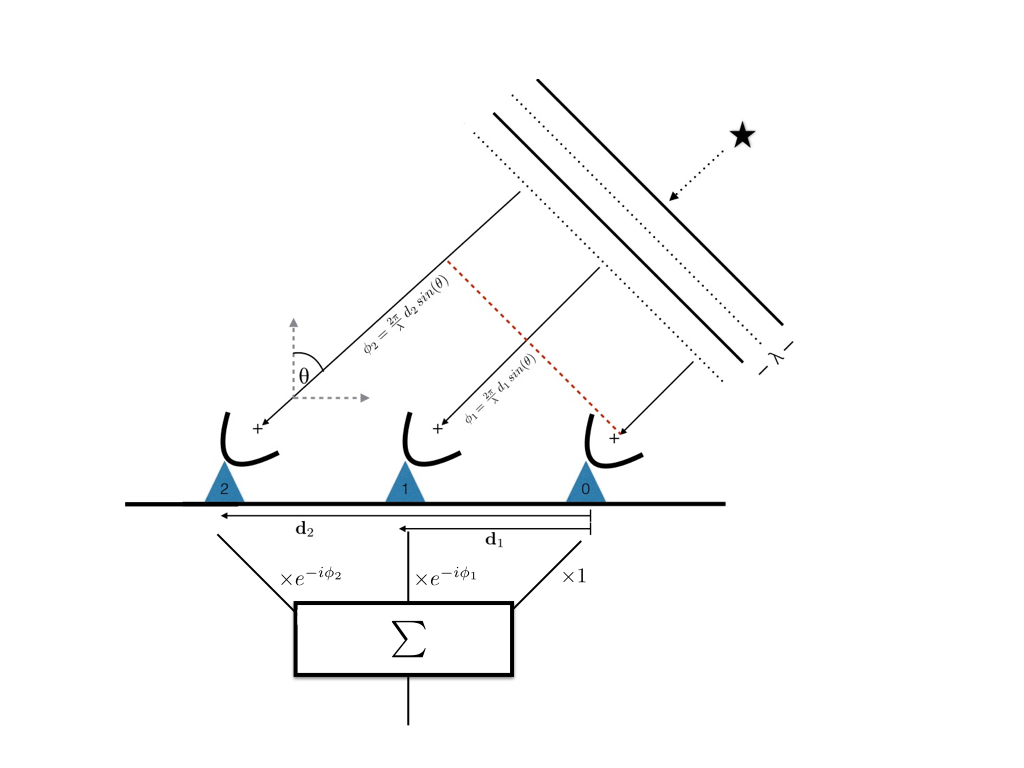
\includegraphics[trim={1.in, 1.in, 2.5in, 1.in}, width=1\textwidth]{./figures/beamforming/beamforming_diagram.jpeg} 
\vspace{0.0cm}
\caption[abc]{Diagrammatic example of a three-element beamformer. The 
wavefront from a far-field point-source arrives at each antenna 
at different times, but the delay is calculable given an array 
configuration and a direction to the object. Complex weights can 
be applied to each antenna's voltage time-stream to account 
for the geometric delay, allowing for the signals to be summed coherently.}  
\vspace{-0.4cm}   
\end{center}
\end{figure}

To calculate the projection $\mathbf{d}_n \cdot  {\mathbf{\hat{k}}}$, we 
need to go from celestial coordinates, in this case equatorial, to geographic 
coordinates. This requires only a source location, an observer location, and an 
observing time. For the latter we use local 
sidereal time (LST), which is the $RA$ of the local meridian. This can be determined  
by an observer's longitude and a time, e.g. a Coordinated Universal Time (UTC). 
A source's hour angle is simply the difference between $LST$ and its $RA$,

\begin{equation}
HA = LST - RA.
\end{equation}

We use the standard interferometric $(u, v, w)$ coordinate system 
to describe our baseline vector, $\mathbf{d}_n$. This is a 
right-handed coordinate system where $u$ (east-west) and $v$ (north-south) are in the plane 
whose normal is the zenith, and $w$ measures the vertical direction \citep{1986isra.book.....T}.
They are defined in numbers of wavelengths, with
$u = d_{\rm ew} / \lambda$, $v = d_{\rm ns} / \lambda$, 
and $w = d_{\rm vert} / \lambda$. Eq.~\ref{eqn-phi_n} can we expanded 
as,

\begin{align}   
\phi_n &= 2\pi \, (u, v, w) \cdot \mathbf{\hat{k}}\\
&= 2 \pi \left ( 
u \, \mathit{\mathbf{\hat{u}}} \cdot \mathbf{\hat{k}} + 
v \, \mathbf{\hat{v}} \cdot \mathbf{\hat{k}} + 
w \, \mathbf{\hat{w}} \cdot \mathbf{\hat{k}} 
\right ),
\end{align}

\noindent where each projection component can be obtained 
using spherical trigonometry. Though we do not go through the
derivation here, it is given by the following product,

\begin{equation}
\label{eq-fringestop_phase}
\mathbf{d}_n \cdot  {\mathbf{\hat{k}}} = \lambda \begin{pmatrix}
u, & v, & w
\end{pmatrix}  \cdot \begin{pmatrix} 
-\mathrm{cos}\delta \,\mathrm{sin}HA \\ 
\, \mathrm{cos}(lat) \, \mathrm{sin}\delta - \mathrm{sin}(lat) \, \mathrm{cos}\delta \, \mathrm{cos}HA \,\\
\, \mathrm{sin}(lat) \, \mathrm{sin}\delta + \mathrm{cos}(lat) \, \mathrm{cos}\delta \, \mathrm{cos} HA\,
\end{pmatrix} .
\end{equation}

These phases are not only essential to beamforming but 
also for the fringestopping process, which is ubiquitous in 
interferometric analysis and is descibed in Sec.~\ref{sec-instr_phases}.


\begin{table}[]
\centering
\label{tab-coord_var}
\begin{tabular}{ll}
\multicolumn{1}{c}{\textbf{Variable}} & \multicolumn{1}{c}{\textbf{Coordinate}} \\ \hline
$\delta$                              & Source declination                      \\
$RA$                                    & Source right ascention                  \\
$LST$                                   & Local sidereal time                     \\
$HA$                                    & Source hour angle                       \\
$alt$                                   & Source altitude                         \\
$az$                                    & Source azimuth                          \\
$lat$                                   & Telescope latitude                      \\
$lon$                                   & Telescope longitude                    
\end{tabular}
\end{table}

\section{Pathfinder beamformer}

\subsection{Instrumental phases}
\label{sec-instr_phases}
In a real experiment, if the voltages from each antenna, $x_n$, are summed 
without any adjustment as written in Eq~\ref{eq-bf_sum}, one should only 
expect noise and not a coherent beam. This is because we have assumed 
the wavefront's differential time-of-arrival across at array 
is the same time delay seen by the correlator. In fact each 
signal is further delayed by multiple steps in the signal chain. 
Digital phases in the electronics can be added by the LNAs and FLAs, and
coaxial cables, whose lengths vary by up to a meter, can rotate 
the signal by multiple radians. Therefore in order to coherently sum 
across the array and beamform, the instrumental phases must be removed. 
If $e_n$ is the true electric field on the 
sky as seen by each feed, then the thing we measure is the on-sky signal
altered by an effective gain, $g_n$, and a noise term, $n_n$.

\begin{equation}
     x_n = g_n e_n + n_n
\end{equation}

\noindent We have lumped several terms into $g_n = |g_n| e^{i \phi_{g_n}}$, 
which is composed of a pointing-dependent beam term
and any complex gain introduced after light hits the cylinder. 
Since we really only care about the phase, we can decompose $\arg(g_n)$
as,

\begin{equation}
\phi_{g_n} = \phi_{\rm beam} + \phi_{\rm an} + \phi_{\rm e} + \phi_{\rm fpga} 
\end{equation}

\noindent where $\phi_{\rm beam}$ is the beam's phase for a given pointing, 
$\phi_{\rm an}$ comes from the analogue chain (dual-pol feed, coax, etc.),  
$\phi_{\rm e}$ is any phase introduced in the electronics, 
and $\phi_{\rm fpga}$ are phases applied in the $F$-engine. 

Since the instrumental phases are effectively random, the simplest 
way to remove them is to solve for them empirically, usually from 
a point-source on the sky. Using the visibility definition in 
Eq~\ref{eqn-visibility}, one can evaluate that all-sky integral 
assuming the sky's electric field is produced by a single point-source. 
This is tantamount to a delta function at a single direction on the sky.

\begin{align}
V^{\rm ps}_{m,n} &= \int d^2\mathbf{\hat{k}} \, g_m(\mathbf{\hat{k}}) \, g^*_n(\mathbf{\hat{k}})\, e_m(\mathbf{\hat{k}}) e_n^*(\mathbf{\hat{k}})\, \delta(\mathbf{\hat{k}} - \mathbf{\hat{k}}_{\rm ps})\\
 &= {g}_m(\mathbf{\hat{k}}_{\rm ps}) \, g^*_n(\mathbf{\hat{k}}_{\rm ps})\,e_m(\mathbf{\hat{k}}_{\rm ps}) e_n^*(\mathbf{\hat{k}}_{\rm ps})
\end{align}

\noindent In this equation $\mathbf{\hat{k}}_{\rm ps}$ is the only direction 
on the sky with a source --- an approximation whose validity we 
will discuss below --- and $\delta$ is a Kronecker delta function. 

\begin{equation}
V_{m, n}^{\rm ps} = 
\end{equation}

% This may need to go earlier on in the thesis, perhaps in the intro
% or the CHIME chapter if it exists
\begin{equation}
\label{eqn-visibility}
     V_{m,n} = \int d^2\mathbf{\hat{k}} \,
     g_m(\mathbf{\hat{k}}) \, g^*_n(\mathbf{\hat{k}})\, e_m(\mathbf{\hat{k}}) e_n^*(\mathbf{\hat{k}})
\end{equation}

\noindent If we explicitly write the phase information of the sky's 
electric field, we can use 

\begin{equation}
\label{eqn-tsky}
e_m(\mathbf{\hat{k}}) e_n^*(\mathbf{\hat{k}}) = T(\mathbf{\hat{k}}) 
e^{2\pi \,i \,\mathbf{\hat{k}} \cdot \mathbf{d}_{mn}}.
\end{equation}

\begin{equation}
\label{eqn-visibility-temp}
     V_{m,n} = \int d^2\mathbf{\hat{k}} \,
     g_m(\mathbf{\hat{k}}) \, g^*_n(\mathbf{\hat{k}})\, T(\mathbf{\hat{k}}) 
e^{2\pi \,i \,\mathbf{\hat{k}} \cdot \mathbf{d}_{mn}}
\end{equation}


Therefore a single correlation can be written as an intensity multiplied 
by a phase factor that is determined by the source-position's 
projection onto that correlation's baseline. Since that phase 
factor is calculable via Eq.~\ref{eq-fringestop_phase}, it 
can be removed in a process called ``fringestopping". The 
data can be inspected visually quite easily, since 
a transiting point-source will fringe as a function of 
time at a rate corresponding 
to the projected baseline length, but should not after fringestopping 
is applied. This is demonstrated with an inter-cylinder Cygnus A transit in 
Fig.~\ref{fig-fringestop}. 

% -------------------------------------------- FIGURE 1 --------------------------------------------

\begin{figure}[!h]
\label{fig-fringestop}
\begin{center}
\vspace{1cm}
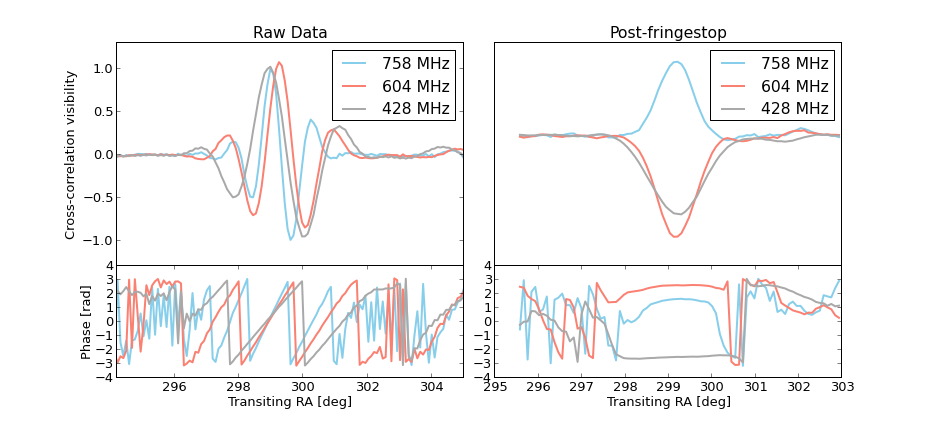
\includegraphics[trim={1in 0in 1in 1in}, width=\smwidth]{./figures/beamforming/thesis_fringestop.png}
\caption[abc]{An example of the fringestopping process that is 
 necessary for gain calibration off of a transiting point-source. Since 
 the phase of a visibility will have a time- and frequency-dependent 
 component, the measured correlation will fringe as the earth rotates in 
 a chromatic way. This effect can be removed by multiplying each visibility by 
 $e^{-i \phi_{\rm mn}(\rm t, \nu)}$, as determined by Eq.~\ref{eq-fringestop_phase}. 
 The top left panel shows the raw correlation as a function of transiting
 $RA$ between feeds 1 and 129, which are of the same polarization but 
 on opposite cylinders, separated by 21 m. We plot  
 three different frequencies. The panel below it 
 shows the same complex visibility's phase. The slope, or fringe-rate, decreases 
 at lower frequencies, as expected. The right panel show the same data 
 after running it through the fringestopping pipeline. Though the resulting 
 phases are near flat, implying that the baseline is no long fringeing, 
 the visibilities are not purely real; this is because there are residual 
 instrumental phases. These phases can be solved for using an 
 eigendecomposition now that the array is phased up to a single point-source.}  
\end{center}
\end{figure}

% -------------------------------------------- FIGURE 1 --------------------------------------------


The $N(N+1)/2$ visibilities we measure can be thought of as 
the upper triangle of an $N\times N$ complex Hermitian 
matrix, $\mathbf{V}$. This is simply the outer product of the 
signal vector, $\mathbf{x}$, with its Hermitian conjugate. 

\begin{align}
\label{eqn-corrmat}
\mathbf{V} = \mathbf{x} \mathbf{x}^\dagger &\approx \begin{pmatrix}
|g_0|^2\, e_0^2 &  & ... & & & \\ 
 &  &  & &  g_n g_m^* e_n e_m^*& \\ 
 &  &  \ddots & & & \\ 
 &  &  &  & & \\
&&&&&&\\
 &  &   &  & &  |g_N|^2 \, e_N^2
\end{pmatrix}
\end{align}

If the sky is composed of a single point-source
then this matrix will be rank one, i.e. there is only one 
non-zero eigenvalue. One can see this by referring to Eq.~\ref{eqn-tsky} 
and noting that if the data has been fringestopped, then the 
sky temperature can be factored out of
Eq.~\ref{eqn-corrmat}, which becomes

\begin{equation}
\mathbf{V} = T(\mathbf{\hat{k}}) \, \mathbf{g} \mathbf{g}^\dagger.
\end{equation}

\noindent Therefore by diagonalizing the correlation matrix $\mathbf{V}$ 
we get a complex eigenvector corresponding to the largest 
eigenvalue, that is proportional to the gain vector $\mathbf{g}$. 
The phase of this eigenvector will be an estimate for the instrumental 
phases, $\phi_{g_n}$, up to some unknown global offset. The goodness 
of this calibration depends on the validity of our assumption 
that the correlation matrix is rank one. We can estimate the 
error on the calibration solution as the ratio of the second largest 
eigenvalue, $\lambda_2$, to the largest, $\lambda_1$. For typical 
frequencies we get values of $\frac{\lambda_2}{\lambda_1}\sim3\%$.


These algorithms have been implemented in a pre-beamforming 
pipeline written in {\tt Python}. Each day a point-source transit 
is fringestopped and a calibration solution is solved for. 
The source chosen depends on the solar time of its transit: Since the
sun is extraordinarily bright in our band, the transit has to be 
at night for good calibration solutions. Historically, 
we have used Cygnus A in the spring and summer, Cassiopeia A 
in the summer and fall, and Tau A in the winter. 
Whatever we calibrate off of, the phases of that solution are 
written to pickle files that are readable by the Pathfinder's FPGAs.
The FPGA then applies complex gains after channelization, which 
in theory should provide the beamforming kernel with voltages 
whose phases are purely geometric. 

\section{FRB VLBI search}


\begin{figure}[!h]
\label{fig-bf_diagram}
\begin{center}
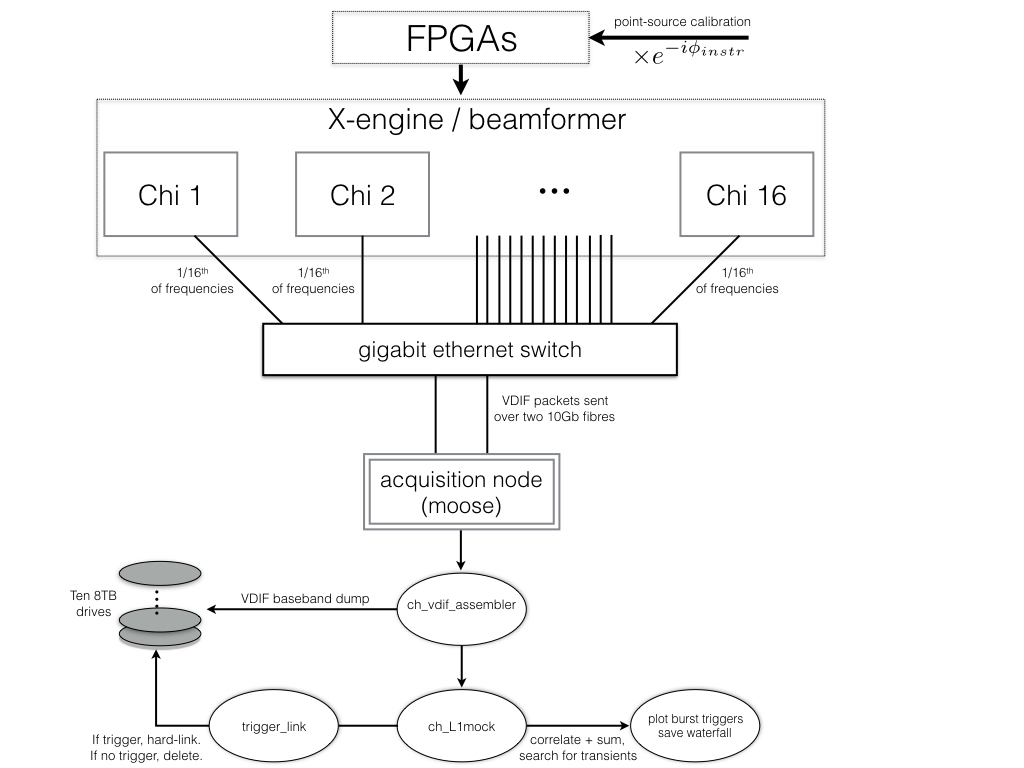
\includegraphics[trim={1.in, 0in, 2.5in, 0in}, width=1\textwidth]{./figures/beamforming/moose_diagram.png} 
%\vspace{0.0cm}
\caption[abc]{Block diagram of the beamforming backend on CHIME Pathfinder. 
A calibration solution is obtained from a bright point-source transit, 
the phases of which are fed into the FPGAs where they are applied as a 
digital gain. All antenna signals are then sent the $X$-engine, 
comprised of 16 GPU nodes. Each node applies geometric phases then 
sums the voltage stream across all antennas with the same polarization. 
The two resultant beams are then sent to our acquisition machine {\tt moose} 
as {\tt VDIF} packets, where a multi-threaded capture code, {\tt ch\_vdif\_assembler}. 
At this point the baseband data are either written to disk as scrambled baseband 
{\tt VDIF}, or they are reorganized in time and frequency. The ordered data are 
searched for FRBs after squaring and integrating to $\sim$millisecond cadence 
using a tree-dedispersion algorithm. If there is a trigger, then the corresponding 
baseband data is hard-linked. Old files that haven't been hard-linked are deleted
periodically.}
\vspace{0.4cm}   
\end{center}
\end{figure}

\section{Conclusion}
\label{sec:conclusion}
  

% ================================================================================
% ACKNOWLEDGEMENTS
% ================================================================================

\section*{\centering Acknowledgements}

We thank Ondrej and Nolan and Peterman.
  
